\section*{ANALYSIS}\label{analysis}
\subsection*{FNPF}\label{fnpf}
The FNPF results have the benifit of having all the three states:
$\phi$, $\dot{\phi}$ and $\ddot{\phi}$. This means that these time
series can be inserted into the differential equation
(Eq.\ref{eq:roll_decay_equation_quadratic_a}) and the parameters
of the model can be estimated using linear regression with Ordinary
Least Square method (OLS), solving the following regression:
\begin{equation}
y = X \cdot \beta + \epsilon
\label{eq:ols}
\end{equation}
where:
\begin{itemize}
\item $y$ is the dependent variable (also called *label*).
\item $\beta$ is a vector with the regressed parameters.
\item $X$ is a matrix containing the independent variables (also called *features*).
\end{itemize}
The roll decay equation can be expressed as a linear regression with
\begin{itemize}
\item $y$ : the roll angle acceleration $\ddot{\phi}$
\item $\beta$ : contains all the parameters : $B_1$, $B_2$, $C_1$...
\item $X$ : contains all the time varying features such as: $| \dot{\phi} | \dot{\phi} $ etc.
\end{itemize}
The roll acceleration is put on the left hand side:
\begin{equation}
\begin{aligned}
- \ddot{\phi} = B_{1A} \dot{\phi} + B_{2A} \left|{\dot{\phi}}\right| \dot{\phi} + B_{3A} \dot{\phi}^{3} + C_{1A} \phi + C_{3A} \phi^{3} \\ + C_{5A} \phi^{5}
\end{aligned}
\label{eq:acceleration_equation_cubic}
\end{equation}
The equation for the acceleration
Eq.\ref{eq:acceleration_equation_cubic} can now be rewritten as
a linear regression (see in Eq.\ref{eq:ols}) where $\beta$,
$X$ and $y$ contain the following:
\begin{equation}
\beta = \left[\begin{matrix}B_{3A}\\C_{3A}\\C_{5A}\\B_{2A}\\B_{1A}\\C_{1A}\end{matrix}\right]
\label{eq:eq_beta}
\end{equation}
\begin{equation}
X = \left[\begin{matrix}\dot{\phi}^{3} & \phi^{3} & \phi^{5} & \left|{\dot{\phi}}\right| \dot{\phi} & \dot{\phi} & \phi\end{matrix}\right]
\label{eq:eq_X}
\end{equation}
\begin{equation}
y = - \ddot{\phi}
\label{eq:eq_y}
\end{equation}
The coefficients determined with Ordinary Least Square fit is shown in
Tab.\ref{tab:parameters_one}. The mean value of these
coefficients are presented togehter with 5\% confidence level
intervalls.
\begin{table}[H]
\scriptsize
\center
\caption{Parameters estimation cubic model (% confidence)}
\label{tab:tab:parameters_one}
\begin{tabular}{|l|l|l|l|l|}
\hline\addlinespace
coeff & mean & $P_{value}$ & $conf_{lower}$ & $conf_{higher}$\\
B_3A & 0.098 & 0.0 & 0.072 & 0.124\\
\hlineC_3A & -5.522 & 0.0 & -5.807 & -5.236\\
C_5A & 254.093 & 0.0 & 244.923 & 263.264\\
B_2A & -0.062 & 0.0 & -0.076 & -0.047\\
B_1A & 0.016 & 0.0 & 0.014 & 0.018\\
C_1A & 6.116 & 0.0 & 6.114 & 6.118\\
\hline
\end{tabular}
\end{table}
\subsection*{Simulation}\label{simulation}
Fig.\ref{fig:sim_cubic} shows a simulation with the regressed
parameters together with the original data from the FNPF simulations.
The simulations are conducted by solving the intial value problem by
Runge Kutta integration of
Eq.\ref{eq:acceleration_equation_cubic}.
\begin{figure}[H]
\begin{center}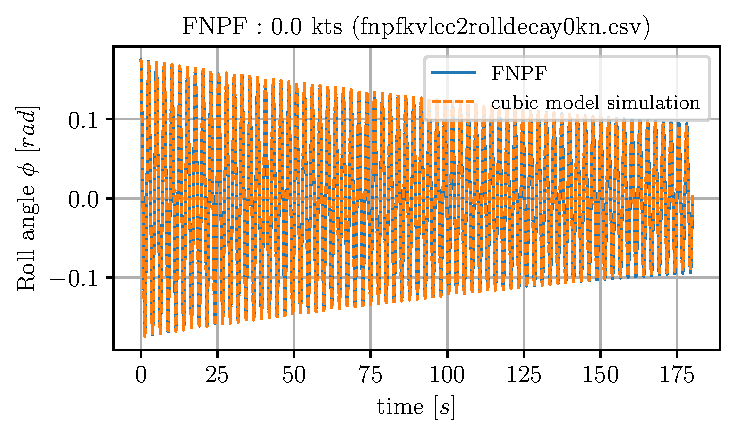
\includegraphics[width = 0.95\textwidth]{figures/sim_cubic.pdf}\end{center}
\vspace{-0.7cm}
\caption{Simulation of roll decay test with parameters from the cubic model.}
\label{fig:sim_cubic}
\end{figure}
The $P_{value}$ is shown for each parameter in
Tab.\ref{tab:parameters_one} testing the null hypothesis $H_0$
for each parameter. $H_0$ tests the probability that a certain
parameter would be 0 (so that it can be removed). For this case the
$P_{value}$ is close to 0 for all parameters, which means that none of
them should be removed.
It can however be noted that the lower and upper limits of the
\textbackslash5\% confidence intervalls differs quite a bit. In the
following, a simpler linear model will therefore also be investigated,
to see if there is a need to reduce the complexity of this model. For a
linear model, the differential equation for the roll motions is reduced
to:
\begin{equation}
- \ddot{\phi} = B_{1A} \dot{\phi} + C_{1A} \phi
\label{eq:Eq(-Derivative(phi(t), (t, 2)), B_1A*Derivative(phi(t), t) + C_1A*phi(t))}
\end{equation}
The $\beta$ and $X$ is now expressed as:
\begin{equation}
\beta = \left[\begin{matrix}B_{1A}\\C_{1A}\end{matrix}\right]
\label{eq:eq_beta2}
\end{equation}
\begin{equation}
X = \left[\begin{matrix}\dot{\phi} & \phi\end{matrix}\right]
\label{eq:eq_X2}
\end{equation}
The parameter estimation for the linear model is shown in
Tab.\ref{tab:parameters2}. It can be noted that the upper and
lower limits of the confidence intervalls are now much closer to each
other. A simulation with this linear model is shown in
Fig.\ref{fig:sim_linear}.
\begin{table}[H]
\scriptsize
\center
\caption{Parameters estimation linear model (5\% confidence)}
\label{tab:tab:parameters2}
\begin{tabular}{|l|l|l|l|l|}
\hline\addlinespace
coeff & mean & $P_{value}$ & $conf_{lower}$ & $conf_{higher}$\\
B_1A & 0.007 & 0.0 & 0.007 & 0.007\\
\hlineC_1A & 6.101 & 0.0 & 6.1 & 6.101\\
\hline
\end{tabular}
\end{table}
\begin{figure}[H]
\begin{center}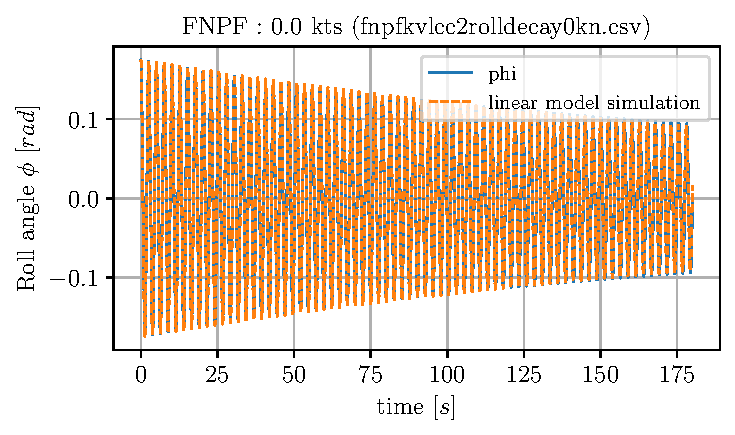
\includegraphics[width = 0.95\textwidth]{figures/sim_linear.pdf}\end{center}
\vspace{-0.7cm}
\caption{Simulation of roll decay test with parameters from the linear model.}
\label{fig:sim_linear}
\end{figure}
The coefficient of determination $R^2$ is very similar between the
cubic (0.997) and the linear model (0.989), when comparing simulated
roll signal with the corresponding data from FNPF.
\subsection*{Model tests}\label{model-tests}
Fig.\ref{fig:roll_decay_model_test} shows the roll signal from
one of the roll decay model tests. A sample from this signal as
indicated by the ``cut'' in Fig.\ref{fig:roll_decay_model_test}
is used to regress the roll damping. The roll velocity and acceleration
are however missing from this model test data. This means that the
regression approach as used for the FNPF data cannot be used directly.
Instead the velocity and acceleration are first estimated using
numerical differentiation. The acceleration and velocity signals
estimated in this way are very noisy as shown in
Fig.\ref{fig:roll_velocity_and_acceleration}, where the roll
angle measurement noise is included in the differentiation. The roll
signal has been low pass filtered prior to the differentiation. The
signal has been filtered using a linear digital filter twice: once
forward and once backwards. This ``filt-filt'' approach ensures that the
filter is not introducing a phase lag onto the signal, which is crucial
for the present regression. A 5th order digital filter with 15 Hz cutoff
frequency was used for the filtering.
Results from a regression with this noisy data is shown in
Fig.\ref{fig:roll_acceleration_ols}, where the numerical
acceleration and a 5\% confidence intervall is also shown.
Fig.\ref{fig:roll_acceleration_residual} shows the residual
distribution. This distribution seems to be approximatelly normal
distributed, which is confirmed when also looking at the normal
probability plot in
Fig.\ref{fig:residual_normal_probability_plot}.
\begin{figure}[H]
\begin{center}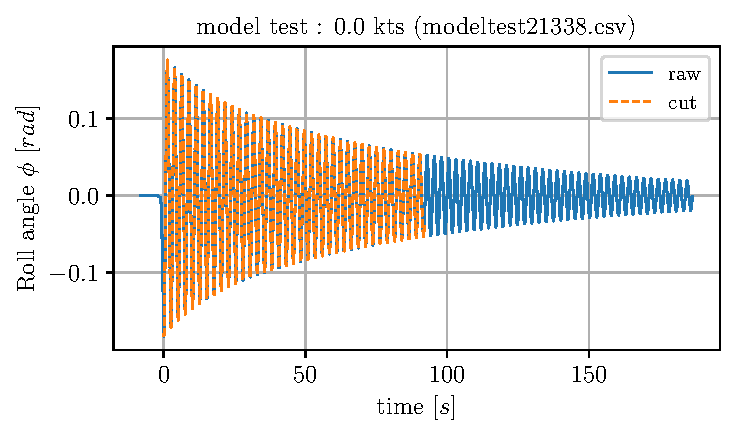
\includegraphics[width = 0.95\textwidth]{figures/roll_decay_model_test.pdf}\end{center}
\vspace{-0.7cm}
\caption{Roll decay model test}
\label{fig:roll_decay_model_test}
\end{figure}
\begin{tcolorbox}[breakable, size=fbox, boxrule=.5pt, pad at break*=1mm, opacityfill=0]
\begin{Verbatim}[commandchars=\\\{\}]
<class 'statsmodels.iolib.summary.Summary'>
"""
OLS Regression Results
================================================================================
=======
Dep. Variable:                  phi2d   R-squared (uncentered):
0.830
Model:                            OLS   Adj. R-squared (uncentered):
0.830
Method:                 Least Squares   F-statistic:
2.243e+04
Date:                Wed, 02 Jun 2021   Prob (F-statistic):
0.00
Time:                        09:50:33   Log-Likelihood:
1831.1
No. Observations:                9193   AIC:
-3658.
Df Residuals:                    9191   BIC:
-3644.
Df Model:                           2
Covariance Type:            nonrobust
==============================================================================
coef    std err          t      P>|t|      [0.025      0.975]
------------------------------------------------------------------------------
B\_1A           0.0322      0.012      2.758      0.006       0.009       0.055
C\_1A           6.1152      0.029    211.792      0.000       6.059       6.172
==============================================================================
Omnibus:                      187.004   Durbin-Watson:                   0.564
Prob(Omnibus):                  0.000   Jarque-Bera (JB):              406.315
Skew:                           0.018   Prob(JB):                     5.88e-89
Kurtosis:                       4.029   Cond. No.                         2.47
==============================================================================
Notes:
[1] R� is computed without centering (uncentered) since the model does not
contain a constant.
[2] Standard Errors assume that the covariance matrix of the errors is correctly
specified.
"""
\end{Verbatim}
\end{tcolorbox}
\begin{table}[H]
\scriptsize
\center
\caption{Parameters estimation cubic model}
\label{tab:tab:parameters3}
\begin{tabular}{|l|l|l|l|l|}
\hline\addlinespace
coeff & mean & $P_{value}$ & $conf_{lower}$ & $conf_{higher}$\\
B_3A & -0.133 & 0.918 & -2.65 & 2.385\\
\hlineC_3A & 7.441 & 0.583 & -19.155 & 34.037\\
C_5A & -88.159 & 0.847 & -981.645 & 805.328\\
B_2A & 0.132 & 0.843 & -1.177 & 1.441\\
B_1A & 0.009 & 0.913 & -0.149 & 0.166\\
C_1A & 6.046 & 0.0 & 5.887 & 6.205\\
\hline
\end{tabular}
\end{table}
\begin{table}[H]
\scriptsize
\center
\caption{Parameters estimation linear model}
\label{tab:tab:parameters4}
\begin{tabular}{|l|l|l|l|l|}
\hline\addlinespace
coeff & mean & $P_{value}$ & $conf_{lower}$ & $conf_{higher}$\\
B_1A & 0.032 & 0.006 & 0.009 & 0.055\\
\hlineC_1A & 6.115 & 0.0 & 6.059 & 6.172\\
\hline
\end{tabular}
\end{table}
\begin{figure}[H]
\begin{center}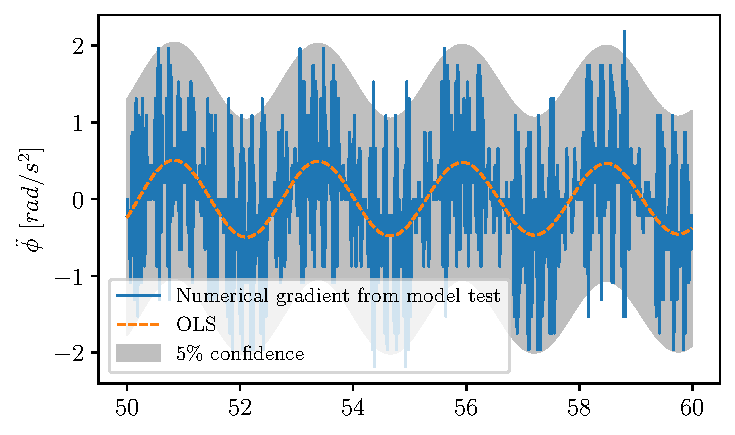
\includegraphics[width = 0.95\textwidth]{figures/roll_acceleration_ols.pdf}\end{center}
\vspace{-0.7cm}
\caption{Roll acceleration from numerical gradient and OLS regression}
\label{fig:roll_acceleration_ols}
\end{figure}
\begin{figure}[H]
\begin{center}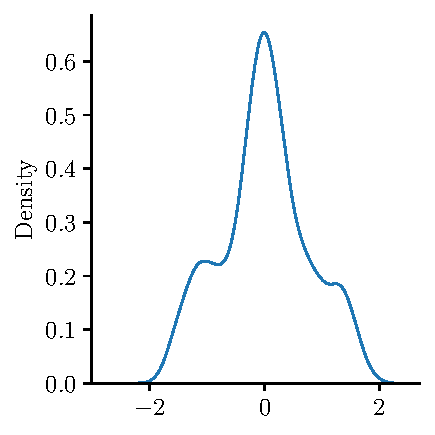
\includegraphics[width = 0.95\textwidth]{figures/roll_acceleration_residual.pdf}\end{center}
\vspace{-0.7cm}
\caption{Roll acceleration residual of linear model}
\label{fig:roll_acceleration_residual}
\end{figure}
\begin{figure}[H]
\begin{center}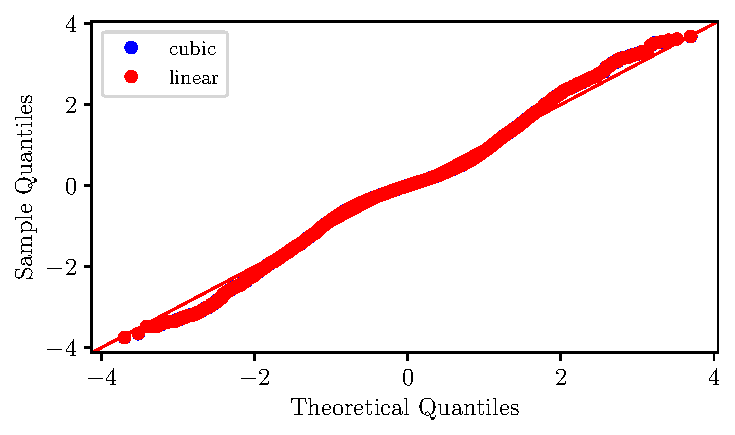
\includegraphics[width = 0.95\textwidth]{figures/residual_normal_probability_plot.pdf}\end{center}
\vspace{-0.7cm}
\caption{Residual Normal probability plot}
\label{fig:residual_normal_probability_plot}
\end{figure}
The coefficient of determination $R^2$ is slightly higher for the
cubic model (0.997) compared to the the linear model (0.982), when
comparing simulated roll signal with the corresponding data from the
model test.
\subsection*{Validation}\label{validation}
The other model test at 0 knots (see
Fig.\ref{fig:other_roll_decay}) is used for validation of the
regression models.
\begin{figure}[H]
\begin{center}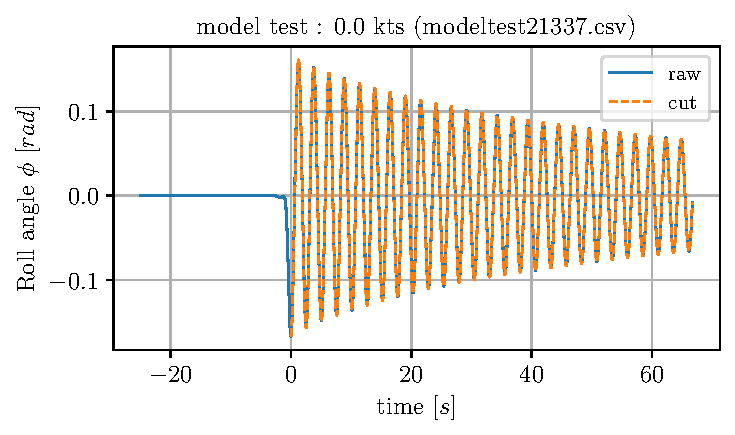
\includegraphics[width = 0.95\textwidth]{figures/other_roll_decay.pdf}\end{center}
\vspace{-0.7cm}
\caption{The other roll decay model test at 0 knots}
\label{fig:other_roll_decay}
\end{figure}
Fig.\ref{fig:other_roll_decay_sim} shows a comparison with this
model test and simulations with regressed parameters from the first
model test.
\begin{figure}[H]
\begin{center}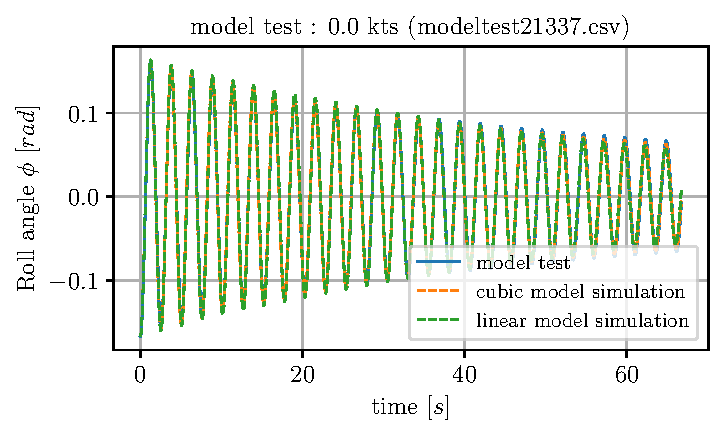
\includegraphics[width = 0.95\textwidth]{figures/other_roll_decay_sim.pdf}\end{center}
\vspace{-0.7cm}
\caption{The other roll decay model test compared with corresponding simulations with linear and cubic models regressed from the first model test.}
\label{fig:other_roll_decay_sim}
\end{figure}
The coefficient of determination $R^2$ is similar for the cubic model
(0.998) compared to the the linear model (0.992), when comparing
simulated roll signal with the corresponding data from the model test.
